\documentclass{llncs}
\usepackage{epsfig,endnotes,comment}
\usepackage[hyphens]{url}

\title{Minimizing Web Latency via Network Aware DNS Redirections from Client Devices}

\author{Utkarsh Goel \and Mike P. Wittie \and Qing Yang}
%
\authorrunning{Utkarsh Goel et al.} % abbreviated author list (for running head)
%
%%%% list of authors for the TOC (use if author list has to be modified)
\tocauthor{Utkarsh Goel, Mike P. Wittie, and Qing Yang}
%
\institute{Department of Computer Science,\\
Montana State University, Bozeman MT 59715,\\
\email{\{utkarsh.goel, mwittie, qing.yang\}@cs.montana.edu}
}


\begin{document}
\maketitle

\begin{abstract}

\end{abstract}


\section{Introduction}

%% SP

The growing popularity of Web based applications such as online social networking, e-commerce, etc, has driven the interest of developers towards improving responsiveness of Web applications.
Recent studies show that application deployment strategies, including the use of Content Delivery Networks~(CDNs), play a vital role in influencing the application performance and the user experience~\cite{cdnbenefitsRackspace}\cite{cdnbenefitsCdnnetworks}.
To increase responsiveness and satisfy customer needs, online businesses invest huge monetary resources into their application deployment and ensure that their services will attract and retian users in long run~\cite{oreilly:businessloss}\cite{server:queue}\cite{blogspot:marissa}\cite{tabb:businessloss}.
As such, most of the online businesses take advantage of geographically distributed CDN infrastructure to deliver services from servers closest to users.
However, in spite of high monetary investment, user frustration with Web content delivery indicates that CDN performance is far from expected.


%% TP

The static content delivery on Web is largely affected by the network latency between clients and CDN servers~\cite{GoelAppPerfSurvey}\cite{doc:latency}\cite{igvita:latency}.
One of the most critical reasons behind slow Web performance is the presence of multiple round trips between a client and a CDN server.
Current Web page designs offer rich user interactions and therefore downloading such a Web page consists of multiple HTTP GET requests.
These requests usually download images, advertisements, external Javascripts and CSS files.
Further, each of these Web request may consist of a TCP handshake and an HTTP GET request, which results in downloading the desired Web content.
Therefore, application developers strive to reduce the delay in Web content delivery by deploying application content closer to user location.
Inspite of such efforts, the Web content delivery still does not provide the responsiveness that the user desire.
One of the challenges to achieve high responsiveness in Web content delivery is in reducing the unnecessary delay introduced into requests by CDN-DNS load balancing systems. 
CDN systems anounce the server availability to clients using Domain Name Systems~(DNS), based on the traffic-load on each CDN server. 
Existing CDN announcement mechanisms, however, make the CDN-DNS system for static content delivery fail to meet the expectations of user and developer community.

We identified three critical reasons that make CDN-DNS load balancing systems ineffective for static content delivery.
First, when CDN servers are used to ensure high availability and fast delivery of static content, DNS responses for CDN domains contain a list of multiple CDN servers. 
Although, a DNS response may contain a list of nearby CDN servers, our measurment study on CDNs used by Facebook and Google shows that there is a high performance gap between different CDN servers returned in the DNS response.
Second, our measurement study demonstrates that a high performance gap between CDN servers is also accompanied by the choice of DNS server.
That is, the CDN servers returned by one DNS server can perform remarkably better than the CDN servers returned by another DNS server.
And third, large-scale networks (such as university or corporate networks) and user devices are often configured with firewalls, which make some servers inaccessible.
However, servers could also be perceived as inaccessible by clients when servers experience high user traffic and offers low uptime to user requests.
Our study shows that DNS resolutions occasionally redirect client applications to inaccessible CDN servers. resulting in failed downloads of Web content~\cite{facebook:failedimage}\cite{facebook:failedimage1}\cite{facebookfailedimage:techspot}\cite{facebookfailedimage:techsupportforum}.
Therefore, we believe that DNS based techniques to load-balance the user traffic will continue to confine the application performance, until such techniques use live information of last-mile network performance while announcing DNS updates.

%% TS

We understand that if DNS were aware of last-mile performance, they could redirect clients to faster CDN servers and achieve the desired application performance.
However, based on our study to characterize the role of DNS redirections on Web content delivery, we argue that clients are better positioned to measure CDN performance than DNS servers.
It is therefore timely to explore solutions where server selection is done by the clients, or through selection mechanisms in the end networks.
We therefore argue that the load balancing functionality must be shared and extended to clients and CDNs. 
We therefore propose DNS-Proxy~(DP), a DNS based proxy that makes network aware DNS redirections based on the performance of network to which it is connected and redirects client devices to potentially fastest CDN server, as it perceives. 
DP relies on a lightweight probing mechanism that probes different CDN servers to find the fastest available and accessible CDN server, before redirecting clients.
To best of our knowledge, DP is the first step in this direction that provides a novel mechanism to extend CDN load-balancing to client devices.
Based on our measurement study on CDNs used by Facebook and Google, we illustrate three contributions of this paper.
First, DP reduces the Web page load time by 40\%.
Second, if a request for a domain is already resolved by DP, the reduction in Web page load time is about 60\%.
Finally, DP reduces the download time of individual Web objects by 70\%.


%% IS

We believe that DP builds the foundation of a new paradigm where load balancing is a shared functionality between CDNs and client devices.
DP will enable application developers and content providers to use their existing infrastructures more effectively.
We believe that a wide adoption of DP in client applications or in last-mile networks will bring significant reductions in the Web page load times and static content delivery.
Even though our study focuses on Web content delivery, we argue that DP will bring significant improvements to the performance of services such as online gaming, collaborative and interactive communications, etc.
Finally, DP is available as an open source tool for application developers and end-user devices\footnote{Public Github Repository: https://github.com/msu-netlab/DNS-Proxy}.

The rest of the paper is organized as follows. 
In Section~\ref{related_work} we outline the related work to reduce the latency in Web communications.
In Section~\ref{discussion}, we showcase the ineffectiveness of CDN/DNS systems.
In Section~\ref{methodology}, we discuss the implementation of DP. 
Finally, we conclude in Section~\ref{conclusions}. 




\section{Related Work}
\label{related_work}

Previous studies have proposed a number of techniques to minimize and understand the impact of network latency on application performance~\cite{GoelAppPerfSurvey14}.
Specifically, some techniques reduce the Web latency through new communication protocols implemented in client browsers and others understand the impact of DNS redirections on application performance.

\subsection{Web based techniques to reduce Web latency}

Shared Dictionary Compression over HTTP~(SDCH)~\cite{w3:sdch} is a communication protocol that relies on inter-response HTTP compression to minimize the amount of data transfer in the network and latency in data delivery.
Although SDCH enables faster access to commonly used Web objects, SDCH has not been widely adopted by developers, likely due to the difficulties of incorporating it in existing Web frameworks, especially for non-established companies. 

SPDY is another communication protocol that relies on concurrent HTTP connections on a multiplexed TCP connection to reduce the latency in Web communication~\cite{spdy:whitepaper}\cite{googledevelopers:spdy}.
Although, SPDY can reduce the Web latency by 50\%, the benefits of SPDY could be realized only if the Web server has more than six resources to offer to the client browser.

Another technique used by developers to reduce the Webpage load time on client browsers is to identify potential Web pages that developers expect their users to visit in future and pre-fetch such Web pages in the background~\cite{google:bandwidthmanagement}.


\subsection{DNS based techniques to reduce Web latency}

Client based tools for sending DNS requests to multiple DNS servers and using the first DNS response that gets received on the client was proposed by Vulimiri~et al.~\cite{VulimiriConext13}.
Although, it reduces the DNS lookup time, the first DNS response may not redirect the user to the fastest server available and may negate the effect of fast DNS resolutions. 

Namehelp Mobile is a tool that measures the impact of cellular DNS redirections on mobile application performance and allows users to find DNS servers that may perform faster DNS lookups and faster Web downloads~\cite{RulaNamehelp}.
Although, Namehelp compares the performance of different DNS resolutions, it does not consider the performance servers within a DNS response. 


\section{Load-Balancing by CDN Infrastructure}
\label{discussion}

Modern websites rely on CDN infrastrucutre to speed up content delivery. 
CDNs balance load on their servers using DNS redirections~\cite{cdnloadbalancing:dyn}\cite{trafficdirector:dyn}. 
Load-balancing is based on the user's geographic location, server load, and server availability, among others.
Our measurement study on Facebook and Google CDN servers, from data collected in over 4 months from Seattle~\cite{JustinSeattle} and Dasu~\cite{dasuNSDI13} testbeds, shows that CDN based load-balancing techniques do not apear reliable and adequate for reducing the latency between client devices and CDN servers.
As a result, DNS redirections often do not point clients to the closest or to the least-loaded server and will continue to redirect clients to remarkably slower CDN servers.


\subsection{Performance Variation in CDN Choice}

We believe that the HTTP download times vary significantly for different CDN servers returned by a DNS resolution.
To verify our hypothesis, we setup an experiment on 400 test devices obtained from Seattle and Dasu testbeds combined.
We then configured each test device to send a DNS query to its default or local DNS, Google's public DNS and two open DNS servers to resolve CDNs domains used by Facebook and Google.
Next, the test devices gathered DNS responses and initiated probes to measure the time take in establishing TCP connection, receive first bit of HTTP GET, and the image download time, for each of the CDN servers in DNS responses.


\begin{figure*}
\minipage{0.48\textwidth}
  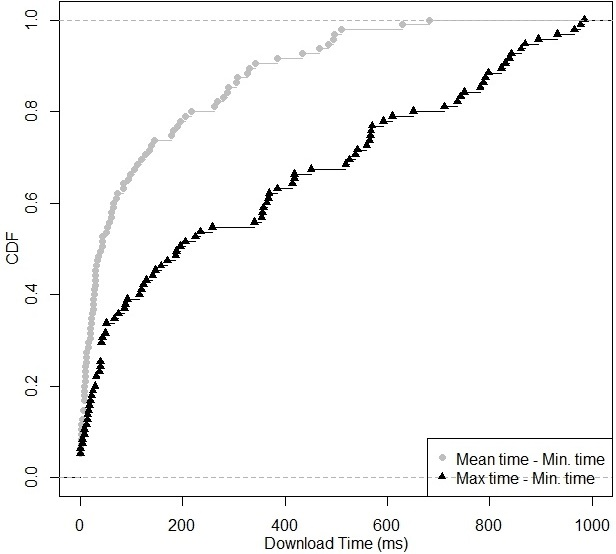
\includegraphics[width=\linewidth]{figures/download_facebook_local_dns}
  \caption{Distribution of image download times based on the choice of Facebook CDN server.}
   \label{fig:download_facebook_local_dns}
\endminipage\hfill
\minipage{0.48\textwidth}%
  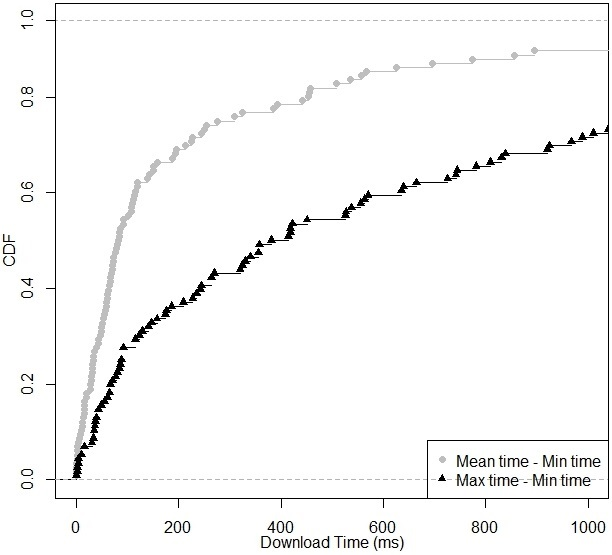
\includegraphics[width=\linewidth]{figures/download_google_local_dns}
  \caption{Distribution of image download times based on the choice of Google CDN server.}
   \label{fig:download_google_local_dns}
\endminipage
\end{figure*}

We depict the variability in image download time from different CDN servers returned by client's local DNS in Figure~\ref{fig:download_facebook_local_dns} and Figure~\ref{fig:download_google_local_dns}.
Figure~\ref{fig:download_facebook_local_dns} shows the variability in download times from Facebook CDN servers, with image download time on x-axis.
Figure~\ref{fig:download_google_local_dns} shows the variability in download times from Google CDN servers, with image download time on x-axis.
The black CDF in both of these figures represents the distribution of the difference of download times between the fastest CDN server and the slowest CDN server, available in the response from client's local DNS.
The grey CDF in both of these figures represents the distribution of the difference of download times between a randomly chosen CDN server and the fastest CDN server, available in the response from client's local DNS.
These graphs show that for most of the clients, the performance of the slowest CDN server in the DNS response is far from the performance of the fastest CDN server available~(also represented by black CDF).
Further, even if the client choses a random CDN server from the DNS response, the download time of the server is higer than the fastest CDN server available~(also represented by grey CDF).
Given the differences in download times, we believe that part of download latency variation comes from the variability in time spent establishing TCP connections and internal server queueing.
We verify these hypothesis next.

%The slow download times are a result of high variablility in latency among different CDN servers to establish TCP connections (due to variable performance of last mile networks) and high variability in HTTP response times (due to variable sizes of request queuing on CDN servers).

Figure~\ref{fig:tcp_open_facebook_local_dns} depicts the the delay of TCP connection establishment with Facebook CDN servers, returned by client's local DNS.
The black CDF represents the distribution of the difference of TCP connection setup times between the fastest CDN server and the slowest CDN server, returned in the DNS response.
The grey CDF in both of these figures represents the distribution of the difference of TCP connection setup times between a random CDN server and the slowest CDN server, returned in the DNS response.
Figure~\ref{fig:tcp_open_facebook_local_dns} shows that for most of the clients, the TCP connection setup time to the slowest CDN server is more than that of the fastest CDN server, available in the DNS response.
We believe that clients have assured opportunity to connect with fastest available CDN server, if DNS were aware of end-user networks.
Therefore, we argue that there is a significant difference in round trip time~(RTT) between a client and different CDN servers returned in a DNS response.

\begin{figure*}
\minipage{0.48\textwidth}
  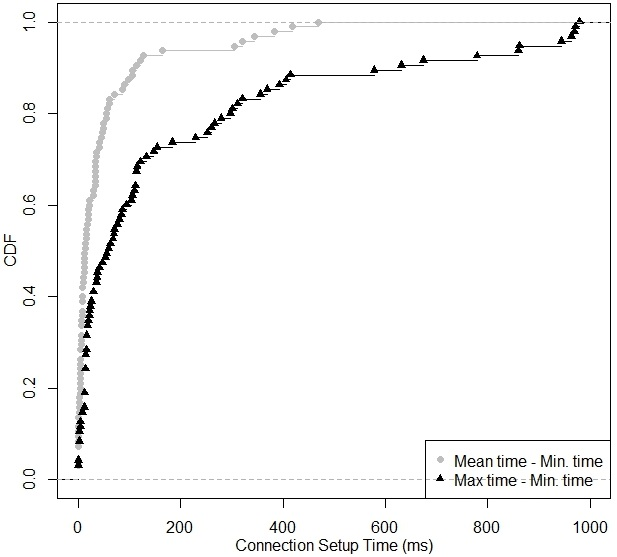
\includegraphics[width=\linewidth]{figures/tcp_open_facebook_local_dns}
  \caption{Distribution of TCP connection setup time to CDN servers used by Facebook.}
  \label{fig:tcp_open_facebook_local_dns}
\endminipage\hfill
\minipage{0.48\textwidth}%
  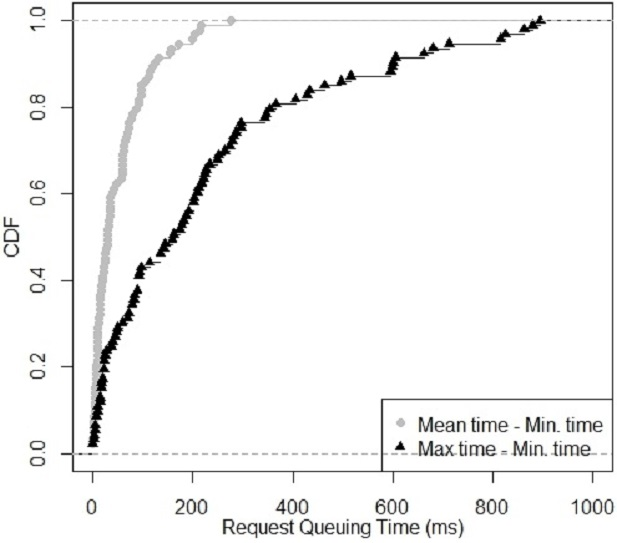
\includegraphics[width=\linewidth]{figures/server_queuing_facebook_local_dns}
  \caption{Distribution of HTTP request queuing time on CDN servers used by Facebook.}
   \label{fig:server_queuing_facebook_local_dns}
\endminipage
\end{figure*}


Finally, request queuing on CDN server plays an additional role in influencing the performance of Web based applications.
A high user traffic on a CDN server could reult in high queueing delays, supplementing the response generation time on the server.
The HTTP HEAD response time~(the time to get the first bit of response) is an ideal indicator of the size of the request queue on a CDN server.
In Figure~\ref{fig:server_queuing_facebook_local_dns}, we depict the  variation in HTTP request queuing on CDN servers used by Facebook.
The black CDF represents the distribution of the difference of HTTP request queuing times between the lowest loaded CDN server and the heavy loaded CDN server, returned in the DNS response.
The grey CDF in both of these figures represents the distribution of the difference of HTTP request queuing time between a randomly chosen CDN server and the heavy loaded CDN server, returned in the DNS response.
We see that CDN servers returned by DNS have different request processing times and thus an inappropriate server selection will increase the HTTP response time, especially when CDN-DNS systems announce inappropriate server availability to end users.



\subsection{Performance Variation with DNS Choice}

Analogous to the choice among CDN servers, clients also have a choice between DNS servers.
Our study shows that a client misses an additional opportunity to reduce the Web latency when it is complelled to use a single DNS server to perform domain name lookups, because the performance of CDN servers returned by one DNS server differs from the performance of CDN servers returned by another DNS server.

%DNS Choice Graphs

\begin{figure*}
\minipage{0.48\textwidth}
  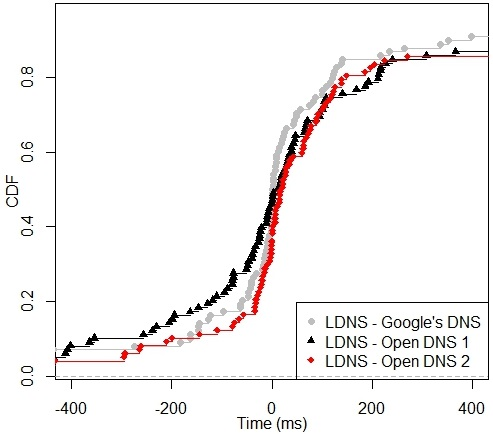
\includegraphics[width=\linewidth]{figures/dns_selection_avg_download_time_facebook}
  \caption{Distribution of image download time for Facebook CDNs based on the choice of DNS server.}
  \label{fig:dns_selection_avg_download_time_facebook}
\endminipage\hfill
\minipage{0.48\textwidth}%
  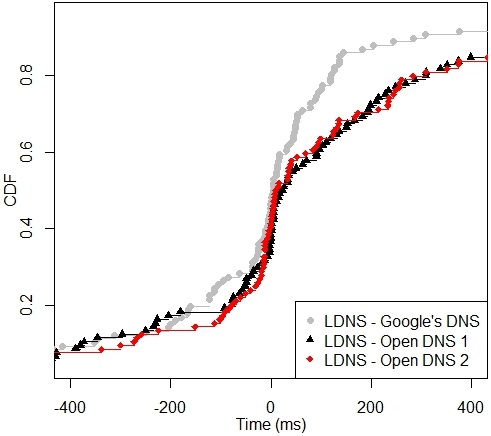
\includegraphics[width=\linewidth]{figures/dns_selection_avg_download_time_google}
  \caption{Distribution of image download time for Google CDNs based on the choice of DNS server.}
  \label{fig:dns_selection_avg_download_time_google}
\endminipage
\end{figure*}

Therefore, we extended our measurement study to evaluate the impact of DNS choice on Web performance.
Specifically, we showcase the impact of DNS choice on image download time in Figure~\ref{fig:dns_selection_avg_download_time_facebook} for Facebook CDN servers and Figure~\ref{fig:dns_selection_avg_download_time_google} for Google CDN servers.
The grey CDF shows a distribution of the difference in the image download times from the fastest CDN server returned by local DNS and the fastest CDN server returned by Google's DNS.
Similarly, red and black CDFs shows a distribution of the difference in the image download times of the fastest CDN server returned by local DNS and the fastest CDN server returned by two Open DNS servers respectively.
We see that client's local DNS server does not return a list with fastest available CDN server, at all times.
For example, for some clients and domain names Google's DNS may return the fastest available CDN server and for other clients and domain names, Open DNS may return the fastest available CDN server.
Therefore, it remains unclear for which client which DNS server will offer the fastest CDN for a given domain. 

We depict similar trends from DNS choice in TCP connection setup time and HTTP request queuing time in Figure~\ref{fig:dns_selection_avg_conn_setup_time_facebook} and Figure~\ref{fig:dns_server_selection_min_request_queue_facebook}, respectively.
Similar to image download time, predicting the CDN server that offers the lowest available TCP connection setup and HTTP request queuing time remains a challenge to low latency Web communication.
Given that the Web performance is affected by the choice of CDN server within a DNS resolution and by the choice of DNS server, it is still unclear how these choice impact the Web performance when combined together.
We believe that it is timely for application developers to understand the combined impact of these choices on application performance and take necessary steps to continue growth in the Web space. 

\begin{figure*}
\minipage{0.48\textwidth}
  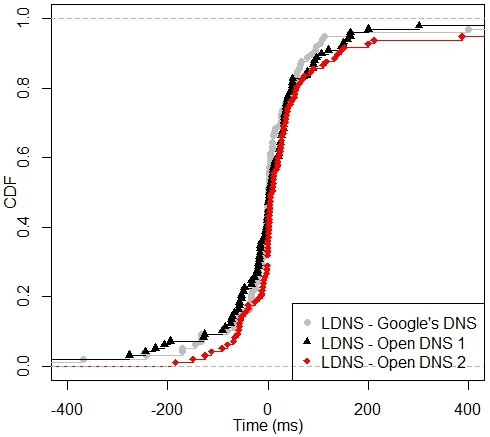
\includegraphics[width=\linewidth]{figures/dns_selection_avg_conn_setup_time_facebook}
  \caption{Distribution of TCP connection setup times for Facebook CDNs based on the choice of DNS server.}
  \label{fig:dns_selection_avg_conn_setup_time_facebook}
\endminipage\hfill
\minipage{0.48\textwidth}%
 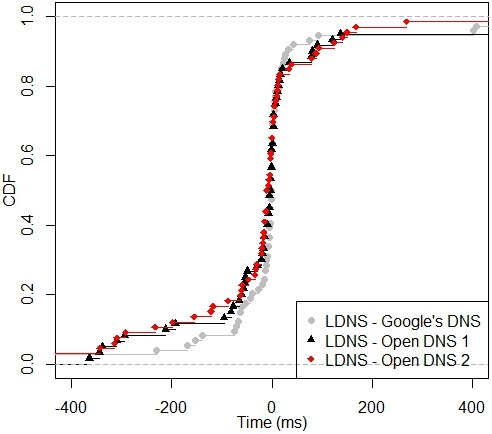
\includegraphics[width=\linewidth]{figures/dns_server_selection_min_request_queue_facebook}
  \caption{Distribution of HTTP request queue time for Facebook CDNs based on the choice of DNS server.}
  \label{fig:dns_server_selection_min_request_queue_facebook}
\endminipage
\end{figure*}


\subsection{Overall Performance Variation}

The impact of CDN and DNS selection is critical on application performance.
Given the performance benefits that accurate CDN and DNS selection brings, we see a high potential for improvement towards Web performance.
In Figure~\ref{fig:download_time_facebook_google_all_dns}, we depict the overall performance gap between the fastest, a randomly chosen, and the slowest available CDN server, obtained from multiple DNS servers. 
The black CDFs represent the download time distribution for Google CDN servers and the grey CDFs represent the performance distribution for Facebook CDN servers.
The CDFs with circular points depict the difference of the download time of the a randomly chosen server and the download time of the fastest server available.
The CDFs with triangular points depict the difference of the download time of the slowest server and download time of the fastest server available. 
From the figure we see that selecting the slowest available CDN server could only match with the latency of the fastest available CDN server for less than only 5\% of the total client devices, whereas, random CDN server could match with the fastest available CDN server for only 20\% of the total client devices.

%Potential for Improvement when multiple DNS are considered

\begin{figure*}
\minipage{0.48\textwidth}
  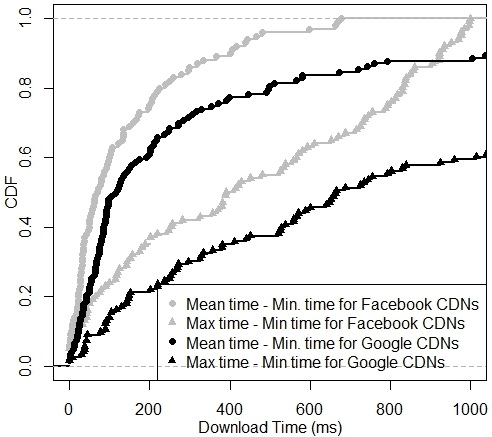
\includegraphics[width=\linewidth]{figures/download_time_facebook_google_all_dns}
  \caption{Distribution of Facebook and Google CDN server latency when responses from multiple DNS servers are considered.}
  \label{fig:download_time_facebook_google_all_dns}
\endminipage\hfill
\minipage{0.48\textwidth}%
  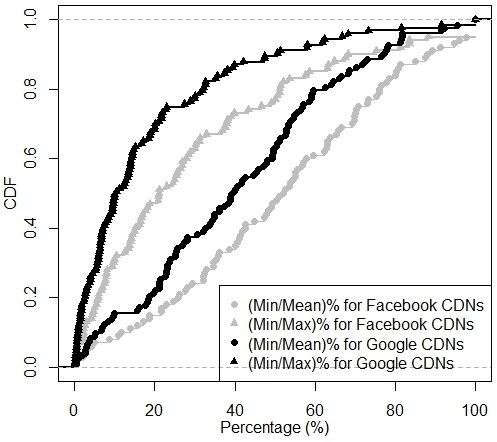
\includegraphics[width=\linewidth]{figures/download_percentage_facebook_google_all_dns}
  \caption{Distribution of Facebook and Google CDN server percentage when responses from multiple DNS servers are considered.}
  \label{fig:download_percentage_facebook_google_all_dns}
\endminipage
\end{figure*}


In figure~\ref{fig:download_percentage_facebook_google_all_dns}, we depict the distribution of overal perfromance gap between CDN servers by percentage.
Similar to figure~\ref{fig:download_time_facebook_google_all_dns}, the black and grey CDFs in figure~\ref{fig:download_percentage_facebook_google_all_dns} represents distribution for Google and Facebook.
The CDFs with circular points represents the ratio of the download time of the fastest server to the download time of a randomly chosen server.
The CDFs with triangular points represents the ratio of the download time of the fastest server to the download time of the slowest server.
In this figure, we show that for Facebook CDN server, the latency of the fastest available server is only about 40\% of the latency of the slowest available CDN server.
However, for Google CDN servers, the latency of fastest server is 60\% of the latency of slowest server.
Compared to the latency of a randomly chosen CDN server, the latency of fastest server is about 80\% for both Facebook and Google.
Therefore, we believe that there is a visible opportunity to reduce the latency in Webpage load time by about 40\%-60\%, which can be realized only if client applications rely on multiple DNS servers for domain name lookups and evaluate the performance of each CDN server before using them. 



\subsection{Network Blockage to Reach CDN Servers}

Client devices and end-networks are often configured with firewalls to block access to certain IP addresses.
Such network configurations are often observed in university or corporate networks.
Such restrictions in the network could be due to automated Intrusion Detection System (IDS) softwares that scan for any activity that might abuse network and device resources.
We verified this as the cause in Montana State University's network.
Such network configurations are unknown to DNS servers and therefore when clients perform DNS lookups, they get redirected inaccessible servers, resulting in failed downloads of Web content~\cite{facebook:failedimage}\cite{facebook:failedimage1}\cite{facebookfailedimage:techspot}\cite{facebookfailedimage:techsupportforum}.
When requested content is not accessible, users get frustrated.
As a result, user interacition with such services decrease~\cite{RadarVelocity09} 
Although, the back-end servers are live, the content availability is usually restricted by firewall and routing configurations in end-networks. 

\begin{figure*}
\centering
\minipage{0.48\textwidth}
  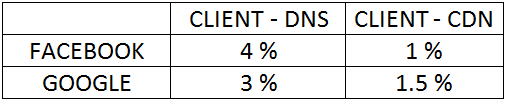
\includegraphics[width=\linewidth]{figures/bad_ip_percentage}
  \caption{Percentage of inaccessible CDN servers.}
  \label{table:bad_ip_percentage}
\endminipage
\end{figure*}

In Figure~\ref{table:bad_ip_percentage}, we depict the percentage of faulty DNS lookups (that is, whether any of the CDN servers in the DNS lookup were identified as inaccessible) and the percentage of inaccessible CDN servers present within any DNS resoultion.
Our measurement study shows that the probability of a DNS server returning a faulty resolution for both Facebook and Google is about 4\% and the chances of an IP address being inaccessible in any DNS resolution are about 1\%.
Although server inaccessibility prevents the content to be downloaded alltogether, we believe that this could be prevented by vetting servers.
We therefore argue that new DNS based mechanims are needed in the end-networks that will check server accessibility of CDN servers before redirecting client applications.


\section{DNS-Proxy}
\label{methodology}

Our study has discovered that CDN/DNS load-balancing system is no-longer reliable and effective in meeting Web application requirements of fast and reliable content delivery.
We see that existing mechanism to load balance the user traffic are not adequate and do not consider the performance of end-networks to which the users are connected.
Therefore, we propose DNS-Proxy (DP), a tool for load-balancing user traffic on CDN servers from client devices in end-networks.
DP extends the CDN load-balancing functionality to client devices and enable users to realize remarkable improvements in page load times and static content delivery in general.

DP operates as a virtual DNS server for client devices and adapts DNS resolutions according to live performance of end-networks.
DP runs as a background service that intercepts DNS requests from client devices. 
A DP installation on a client device will customize DNS redirections based on the performance of client device and it's connectivity with the local network.
DP could also be configured in DHCP to operate as a DNS server on network routers to serve incoming DNS requests from multiple devices in the same network.


\subsection{Network Aware DNS Redirections.}

DP listens for incoming DNS requests on port 53.
When new DNS requests arrive, DP first checks for its local cache to find the fastest available CDN server for the requested domain name.
If the DNS entry for the requested domain name is present in DP's cache, the DNS response is immediately sent to the client.
However, if the DNS entry is not found in the cache, DP establishes a UDP socket to forward the DNS request to multiple DNS servers.
Upon receiving the first DNS response, DP establishes raw sockets and sends TCP SYN packets on port 80 (used by HTTP based services) and port 443 (used by HTTPS based services) of each server in the DNS response.
The performance of each IP address in the DNS response is evaluated based on the time taken to receive a TCP SYN/ACK packet from the server.
Based on the available information about the fastest available CDN server from these measurements, the fastest available IP address for the requested domain name is updated in the DNS entry maintained in the cache.


\begin{figure*}
\minipage{0.48\textwidth}
  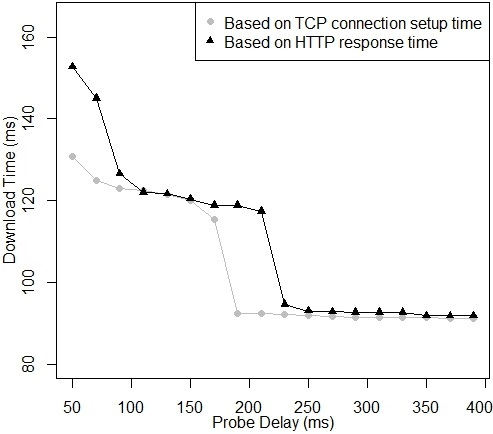
\includegraphics[width=\linewidth]{figures/server_selection_probe_delay_facebook}
  \caption{A comparison of fastest server selection strategy for Facebook CDNs, based on TCP connection setup time, and HTTP response time.}
  \label{fig:server_selection_probe_delay_facebook}
\endminipage\hfill
\minipage{0.48\textwidth}%
  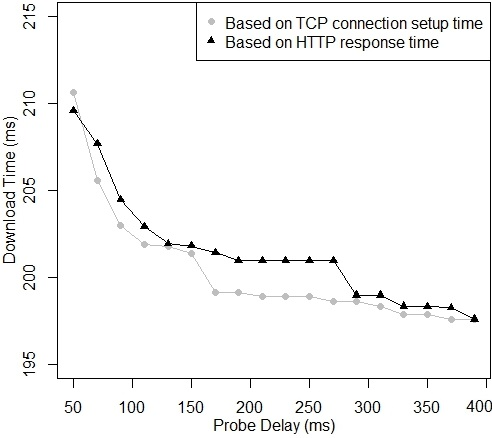
\includegraphics[width=\linewidth]{figures/server_selection_probe_delay_google}
  \caption{A comparison of fastest server selection strategy for Google CDNs, based on TCP connection setup time, and HTTP response time.}
   \label{fig:server_selection_probe_delay_google}
\endminipage
\end{figure*}



\begin{figure*}
\minipage{0.48\textwidth}
  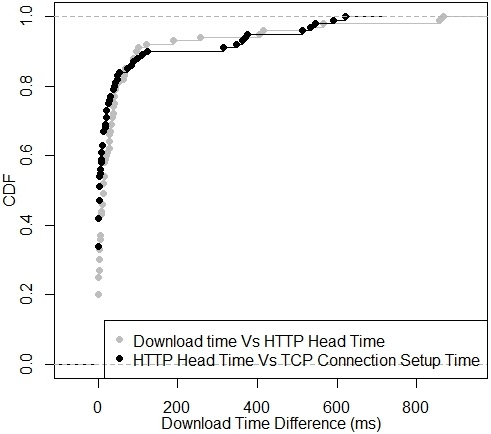
\includegraphics[width=\linewidth]{figures/server_selection_facebook}
  \caption{A comparison of server selection strategy for choosing fastest available Facebook CDN server, based on TCP connection setup time, HTTP response time, and download time of CDNs in DNS response.}
  \label{fig:server_selection_criteria_facebook}
\endminipage\hfill
\minipage{0.48\textwidth}%
  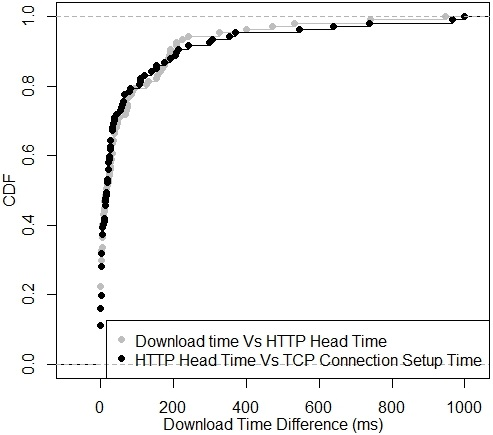
\includegraphics[width=\linewidth]{figures/server_selection_google}
  \caption{A comparison of server selection strategy for choosing fastest available Google CDN server, based on TCP connection setup time, HTTP response time, and download time of CDNs in DNS response.}
   \label{fig:server_selection_criteria_google}
\endminipage
\end{figure*}


Our decision to select TCP connection setup time as an indicative of the CDN performance is based on our measurement data collected from Dasu test devices.
We understand that predicting the fastest available CDN server based on Web content download time will reflect the actual Web performance, however, downloading Web content from each CDN server will require adequate time, which will slow down the overall process to identify the fastest server available and introduce high probing load.
Therefore, we argue that the prediction of fastest available server should be based on faster server selection mechanisms such as HTTP response time or TCP connection setup time between client and server.

We configured experiments on Dasu devices to probe each CDN server, present in DNS resolutions from Google's public DNS, Open DNS, and local DNS, with TCP SYN and by HTTP GET to download an image.
For each experiment between Dasu client and CDN server, we recorded time to establish TCP connection, time to receive first bit of HTTP response, and time to download an image.
Based on the data collected, we found that for a given DNS response containing multiple CDN servers, the image download time offered by the server having least download time is same as the image download time offered by the server having least HTTP response time.
We further found that the download time offered by the CDN server having least HTTP response time is same as the download time offered by the CDN server having the least TCP connection setup time.
Therefore, we argue that TCP connection setup time is equally accurate in predicting CDN performance and should be used to speed up predictions. 
In Figure~\ref{fig:server_selection_criteria_facebook} and Figure~\ref{fig:server_selection_criteria_google}, we compare the three server selection strategies to identify the fastest available server, for Facebook and Google CDN servers respectively.
The grey CDF in both of these figures shows that for more than 80\% of the clients, the difference among image download times offered by the server with the least dowload time and by the server with least HTTP response time is zero. 
The black CDF in both of these figures shows that for more than 80\% of the clients, the difference among image download times offered by the server with the least HTTP response time and by the server with least TCP connection setup time is zero. 
Therefore, with the knowledge that evaluating CDN performance based on TCP connection setup will require lesser time than evaluating CDN performance based on HTTP response time, we decided to speed up DP's processing time involved in CDN performance evaluation, by chosing TCP connection setup time as an indicative of CDN performance.

\begin{figure*}
\minipage{0.48\textwidth}
  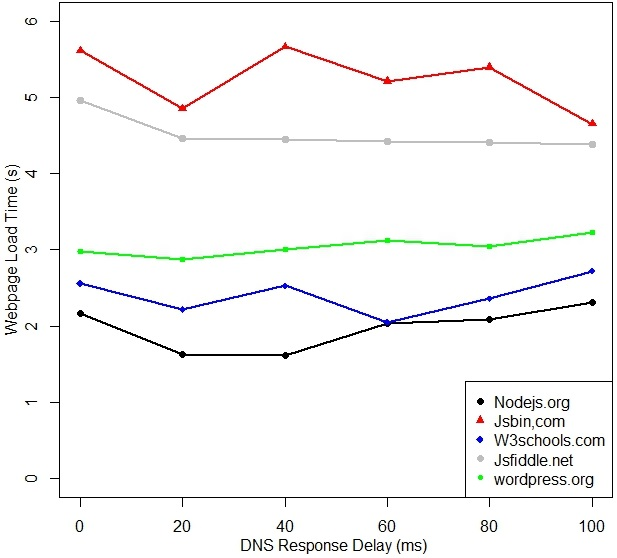
\includegraphics[width=\linewidth]{figures/dns_response_delay}
  \caption{Web page download time of light content Websites when DNS responses are delayed.}
  \label{fig:dns_response_delay}
\endminipage\hfill
\minipage{0.48\textwidth}%
  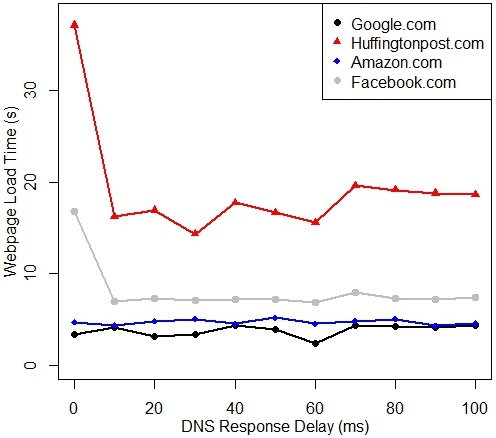
\includegraphics[width=\linewidth]{figures/dns_response_delay_new}
  \caption{Web page download time of heavy content Websites when DNS responses are delayed.}
  \label{fig:dns_response_delay_new}
\endminipage
\end{figure*}

DP can send DNS responses to clients in two different ways.
First, DP could delay the DNS response to allow it to get more time to identify the fastest available CDN server.
And second, DP can replying the client with the first DNS response that it receives from DNS servers.
Although, delaying DNS response appear to inflate the lookup time and the Web latency, our study, however, shows that the overall Web page download time is reduced when clients are redirected to faster CDN servers returned from delayed DNS responses.
For example, In Figure~\ref{fig:dns_response_delay} and Figure~\ref{fig:dns_response_delay_new}, we show that delaying DNS responses by 10ms can reduce the Web page download time by more than 50\% for Websites such as Huffingtonpost.com and Facebook.com.
For other Websites dipicted in these figures, we observed a reduction of more than a second in Web page download time.

Finally, the TTL value of the DNS response from DP is set to 2 seconds.
The benefits of using a low TTL of 2 seconds over a higher TTL value are twofold.
First, it ensures that the client applications will not continue to use the same IP address for a long period of time.
Second, when the client makes the second DNS request after 2 seconds, DP would have already evaluated the performance of different servers, received from multiple DNS servers, and would be able to redirect client devices to a faster CDN server.



\subsection{Elimination of Inaccessible Servers from DNS Redirections.}

Apart from redirecting the end user device to the fastest available CDN server, DP also eliminates any inaccessible Web servers.
However, if a DNS resolution contains only one IP address, DP redirects the user to that IP address, regardless of it being inaccessible.
The process to check whether an IP address is accessible relies on the reply of TCP SYN/ACK from the server.
If a TCP SYN/ACK is received by DP within a timeout period, DP records that IP address as accessible, and innaccessible otherwise.



\subsection{Overall Performance Benefits by using DNS-Proxy}



%Webpage Load Time Graphs

\begin{figure*}
\minipage{0.48\textwidth}
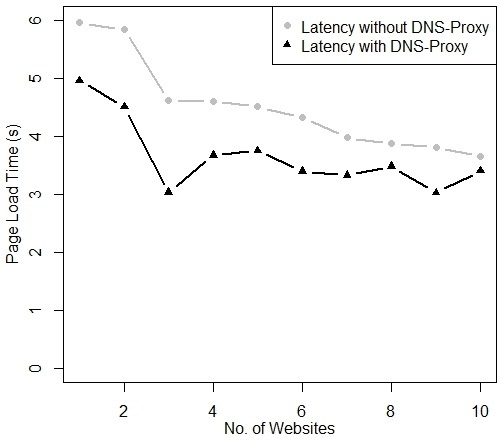
\includegraphics[width=\linewidth]{figures/page_download_time_comparison}
\caption{A comparison of Webpage load times with DNS-Proxy and without DNS-Proxy.}
\endminipage\hfill
\minipage{0.48\textwidth}%
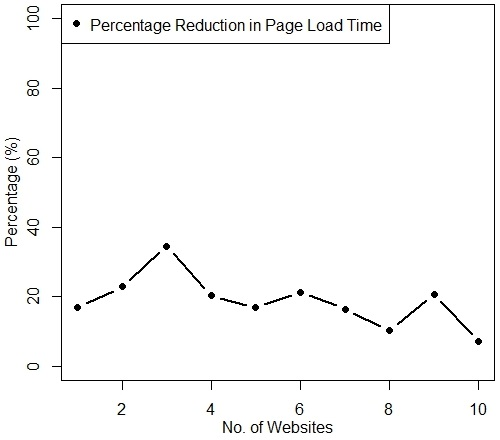
\includegraphics[width=\linewidth]{figures/page_download_percentage}
\caption{Percentage improvement in Webpage load time when DNS-Proxy was used.}
\endminipage
\end{figure*}



\section{Conclusions}
\label{conclusions}

Internet performance is affected by DNS redirections to slow CDN servers, especially when it comes to Web based communication.
Although, it is assumed that DNS resolutions redirect client devices to nearby CDN replicas and that the performance of replicas is similar in performance, our measurement study shows that this is not true.
Based on our extensive evaluation CDN based load-balancing techniques, we discovered a huge performance difference between replicas from intra-response DNS resolutions.
We also discovered that relying upon multiple DNS servers to resolve Internet addresses may redirect client devices to faster CDN replicas.
We, therefore, propose a DNS based proxy (dP) that replicates the CDN based load-balancing on client devices.
Our research is the first step in this direction which pre-determines the performance of every CDN replica resolved by multiple DNS servers and redirect client devices to the fastest available CDN replica.
Based on our measurement study and use of dP, we offer a 20\% - 40\% reduction in Webpage communication.
Finally, we encourage developer community for their participation and wide adoption of this open source tool.

\bibliographystyle{abbrv}

\bibliography{dns_proxy}

\end{document}